%% SoftwareX Article Template
%% ThreatLens: An AI-Assisted DevSecOps Platform for Automated Mobile
%% Application Security Auditing and MASVS v2 Compliance
 
\documentclass[preprint,12pt,a4paper]{elsarticle}
 
\usepackage{amssymb}
\usepackage{amsmath}
\usepackage{hyperref}
\usepackage{listings}
\usepackage{xcolor}
\usepackage{booktabs}
\usepackage{graphicx}
\usepackage{algorithm}
\usepackage{algpseudocode}
\usepackage{tikz}
\usetikzlibrary{shapes.geometric, arrows.meta, positioning, calc, backgrounds, fit}
\setlength{\parindent}{0pt}
 
%% --- TikZ Color Palette (matches Figure 1 & 2 style) ---
\definecolor{tlGreen}{HTML}{2E7D32}
\definecolor{tlGreenLight}{HTML}{E8F5E9}
\definecolor{tlBlue}{HTML}{1565C0}
\definecolor{tlBlueLight}{HTML}{E3F2FD}
\definecolor{tlPurple}{HTML}{6A1B9A}
\definecolor{tlPurpleLight}{HTML}{F3E5F5}
\definecolor{tlOrange}{HTML}{E65100}
\definecolor{tlOrangeLight}{HTML}{FFF3E0}
\definecolor{tlRed}{HTML}{B71C1C}
\definecolor{tlRedLight}{HTML}{FFEBEE}
\definecolor{tlGray}{HTML}{455A64}
\definecolor{tlGrayLight}{HTML}{ECEFF1}
\definecolor{tlGrayDark}{HTML}{263238}
 
\definecolor{codegray}{rgb}{0.95,0.95,0.95}
\definecolor{codeblue}{rgb}{0.13,0.29,0.53}
\lstset{
  backgroundcolor=\color{codegray},
  basicstyle=\small\ttfamily,
  keywordstyle=\color{codeblue}\bfseries,
  breaklines=true,
  frame=single,
  captionpos=b
}
 
\journal{SoftwareX}

\begin{document}
\renewcommand{\labelenumii}{\arabic{enumi}.\arabic{enumii}}

\begin{frontmatter}

\title{ThreatLens: An AI-Assisted DevSecOps Platform for Automated Mobile
Application Security Auditing and MASVS v2 Compliance}
\author[1]{Lahrouf Hiba}
\author[1]{Mahmoud Laasri}

\author[1]{Lachgar Mohamed}

\address[1]{École Marocaine des Sciences de l'Ingénieur (EMSI),
Department of Computer Science, Specialized in Cybersecurity ,
Marrakech, Morocco}

\begin{abstract}
The mobile application ecosystem has grown dramatically, and so has the attack surface it
presents. Security teams face mounting pressure to audit applications against formal standards
such as the OWASP Mobile Application Security Verification Standard (MASVS v2), yet the
volume of findings generated by automated scanners leads to significant alert fatigue and
manual compliance mapping overhead. ThreatLens is a reproducible, open-source DevSecOps
platform designed to orchestrate the mobile application security audit lifecycle. Unlike
standalone scanner integrations, ThreatLens provides a unified orchestration layer that maps
findings from the Mobile Security Framework (MobSF) to MASVS v2 controls, performs
Software Composition Analysis (SCA) via the OSV API, and applies Large Language Model (LLM)
triage through a hybrid deterministic and probabilistic workflow. The platform automatically
assigns CVSS v3.1 scores, generates AI-assisted remediation guidance, and integrates a
Human-in-the-Loop (HITL) review mechanism to preserve expert oversight and continuously
improve triage quality. A dedicated CLI enables integration into CI/CD pipelines as a
security gate. Experimental evaluation on a reproducible corpus of 4 public APKs with
verified SHA-256 hashes demonstrates that ThreatLens achieves a mean audit speedup of
9.2$\times$ compared to manual expert analysis, while maintaining a triage precision of
89.33\%, recall of 95.71\%, and F1-score of 92.41\%. The benchmark dataset, ground-truth
annotations, and reproduction scripts are publicly available in the repository to support
reproducible security research.
\end{abstract}

\begin{keyword}
Mobile Security \sep DevSecOps \sep MASVS v2 \sep OWASP \sep AI-Assisted Triage \sep
Automated Security Auditing \sep LLM \sep CI/CD \sep Software Composition Analysis
\end{keyword}

\end{frontmatter}

%%============================================================
\section*{Required Metadata}
%%============================================================

\section*{Current code version}

\begin{table}[!h]
\centering
\begin{tabular}{|l|p{5.5cm}|p{6.5cm}|}
\hline
\textbf{Nr.} & \textbf{Code metadata description} & \textbf{Information} \\
\hline
C1 & Current code version & v1.0.0 \\
\hline
C2 & Permanent GitHub link to code/repository &
\url{https://github.com/hibalahrouf/ThreatLense.git} \\
\hline
C3 & Legal Code License & MIT License \\
\hline
C4 & Code versioning system used & Git \\
\hline
C5 & Software code languages, tools, and services used &
Python 3.11, FastAPI 0.115.0, Celery 5.4.0, Next.js 16.2.1, React 19.2.4, TailwindCSS, PostgreSQL 16, Redis 7, MobSF v3.9.7, Ollama v0.23.2 (Llama 3 8B Instruct), OpenAI API (GPT-4o), OSV API v1, MinIO \\
\hline
C6 & Compilation requirements, operating environments \& dependencies &
Docker 24+, Docker Compose v2.24+, Python 3.11+, Node.js 18+, 4 vCPUs, 8 GB RAM minimum (16 GB recommended for MobSF dynamic analysis), 20 GB free disk space \\
\hline
C7 & Link to developer documentation/manual &
\url{https://github.com/hibalahrouf/ThreatLense.git/main/README.md}  \\
\hline
C8 & Support email for questions & hibalahrouf@gmail.com\\
\hline
\end{tabular}
\caption{Code metadata (mandatory)}
\label{tab:metadata}
\end{table}

%%============================================================
\section{Motivation and significance}
%%============================================================

Mobile applications have become the primary interface between users and digital services,
processing sensitive data ranging from banking credentials to personal health records.
The attack surface of mobile platforms is consequently enormous: the OWASP Mobile
Application Security Verification Standard (MASVS) enumerates dozens of security
controls across domains including data storage, cryptography, authentication, network
communication, and platform interaction~\cite{owasp_masvs}. Verifying compliance with
these controls is non-trivial: tools such as the Mobile Security Framework
(MobSF)~\cite{mobsf} can generate hundreds of raw findings for a single APK or IPA,
and mapping each finding to a formal MASVS control remains a largely manual,
time-consuming process that demands specialist expertise.

This manual bottleneck creates two compounding problems. First, security auditors spend
a disproportionate fraction of their time on classification and mapping rather than on
expert-level analysis, reducing overall audit throughput. Second, the high volume of
findings promotes \emph{alert fatigue}~\cite{alert_fatigue}, a well-documented phenomenon
in security operations where practitioners begin to ignore or under-triage notifications
because of cognitive overload. Both problems are exacerbated as organisations adopt
continuous deployment practices that demand security feedback on every build.

ThreatLens addresses this gap by introducing a reproducible orchestration layer between raw scanner
output and compliance-ready audit reports. It is positioned not as a replacement for scanners
like MobSF, but as a comprehensive platform for MASVS compliance management, AI-driven triage,
and DevSecOps integration. Its core contribution is a \emph{hybrid triage engine} that combines
deterministic MASVS-mapping rules with LLM-based contextual reasoning to automatically
classify each finding as a True Positive (TP) or False Positive (FP) and to generate a
natural-language justification. This AI-assisted workflow is complemented by a
Human-in-the-Loop (HITL) mechanism: a qualified auditor can review, accept, or override any AI
decision, and each correction is stored in the database as labelled feedback that can be used
for future prompt refinement or model fine-tuning.

From a scientific perspective, ThreatLens provides a reproducible, open-source platform
for studying the effectiveness of LLMs in narrow security domains. Existing research has
demonstrated that large language models can assist in vulnerability detection and code
review~\cite{llm_vuln}, but their integration into formal compliance workflows---with
explainability, auditability, and human oversight---remains underexplored. ThreatLens
operationalises this research direction as a deployable research platform, enabling researchers to
collect labelled triage datasets, measure TP/FP rates across MASVS categories, and
benchmark different LLM backends under identical conditions.

Related tools offer partial coverage. MobSF~\cite{mobsf} excels at static and dynamic
analysis but provides no compliance mapping or AI triage. Commercial platforms such as
NowSecure and Corellium offer managed MASVS assessments but are proprietary, expensive,
and not amenable to research customisation. Open-source static analysis tools such as
Semgrep or Androguard operate at the code level and do not address the compliance
reporting layer. Unlike standalone static analyzers such as MobSF or Semgrep, which require manual mapping of findings to compliance frameworks, ThreatLens introduces an orchestration layer that automatically maps raw scanner output to MASVS v2 controls using a hybrid rule-based and LLM-driven triage engine. To the best of the authors' knowledge, no existing open-source, self-hostable platform combines all of the following in a single pipeline: MobSF-based static and dynamic analysis, automated MASVS v2 control mapping, LLM-assisted TP/FP triage with confidence scoring, HITL auditor feedback, CVSS v3.1 scoring, AI-generated remediation, and native CI/CD integration.

%%============================================================
\section{Software description}
%%============================================================

ThreatLens is implemented as a modular microservices platform designed for horizontal
scalability. The following subsections describe its architecture, major functionalities, and
the core algorithmic process of AI-assisted MASVS mapping.

\subsection{Software architecture}

The architecture of ThreatLens follows an \emph{asynchronous task-driven} pattern,
decomposed into five primary services that communicate over a shared message broker. The overall architecture is illustrated in Figure~\ref{fig:architecture}.

\begin{enumerate}
  \item \textbf{Orchestrator (FastAPI).} The central API gateway handles user
    authentication (JWT), project management, file ingestion, and job
    scheduling. All client requests---from the web dashboard or CLI---are
    processed here. Files are stored in MinIO (an S3-compatible object store)
    to decouple binary storage from application logic.
  \item \textbf{Task Engine (Celery / Redis).} Long-running scan jobs are
    delegated to asynchronous Celery workers via a Redis message broker. This
    decoupling prevents API blocking on large APK files and enables
    horizontal scaling by launching additional workers when queue depth
    increases.
  \item \textbf{Analysis Core.} The analysis core integrates two external
    engines: (a) MobSF~\cite{mobsf}, accessed via its REST API, for static
    analysis (manifest parsing, binary analysis, code scanning) and dynamic
    analysis (instrumented emulator runs); and (b) the OSV
    API~\cite{osv_api} for Software Composition Analysis (SCA), which maps
    extracted third-party libraries to known CVEs and MASVS-CODE-3.
  \item \textbf{AI Triage Engine.} A hybrid engine that processes the raw
    finding list in two passes: a deterministic rule-based pass that maps
    Androguard tags and MobSF issue codes to MASVS v2 controls, followed by
    an LLM inference pass (Ollama / Llama~3 locally, or the OpenAI API for
    cloud deployments) that analyses the code snippet, finding description,
    and MASVS control context to produce a TP/FP classification and a
    natural-language triage justification.
  \item \textbf{Frontend (Next.js 14).} A modern single-page dashboard
    built with Next.js and TailwindCSS provides auditors with project
    management views, an interactive finding list with AI justifications,
    radar charts of MASVS category coverage, and a feedback interface for
    HITL corrections.
\end{enumerate}

All services are containerised with Docker and orchestrated via Docker
Compose, enabling one-command deployment
on any Linux, macOS, or Windows host. The Docker Compose service graph is shown in Figure~\ref{fig:docker}. The PostgreSQL database (managed
with SQLAlchemy and Alembic migrations) stores the full scan lifecycle:
\texttt{User} $\to$ \texttt{Project} $\to$ \texttt{Scan} $\to$
\texttt{Finding} $\to$ \texttt{AuditorFeedback}.

\begin{table}[h]
\caption{Exact component versions used in evaluation}
\begin{tabular}{ll}
Component & Version \\
\hline
MobSF & v3.9.7 \\
Ollama & v0.23.2 \\
LLM Model & Meta Llama 3 8B Instruct (4-bit) \\
PostgreSQL & 16-alpine \\
Redis & 7-alpine \\
MinIO & RELEASE.2024-01-16 \\
FastAPI & 0.115.0 \\
Celery & 5.4.0 \\
Next.js & 16.2.1 \\
React & 19.2.4 \\
Python & 3.11 \\
Docker & 24.0+ \\
Docker Compose & v2.24+ \\
\end{tabular}
\end{table}

\begin{table}[h]
\caption{Primary REST API endpoints}
\begin{tabular}{lll}
Method & Endpoint & Description \\
\hline
POST & /api/auth/register & User registration \\
POST & /api/auth/login & JWT authentication \\
POST & /api/scans/upload & Upload APK, create scan job \\
GET & /api/scans/\{scan\_id\} & Get scan status and progress \\
GET & /api/scans/\{scan\_id\}/findings & Get findings with AI verdicts \\
PATCH & /api/findings/\{finding\_id\}/status & HITL verdict override \\
GET & /api/reports/\{scan\_id\}/pdf & Export PDF compliance report \\
GET & /api/reports/\{scan\_id\}/sarif & Export SARIF file \\
\end{tabular}
\end{table}

Complete interactive API documentation is available at the /docs endpoint (Swagger UI) on any running instance. The raw OpenAPI 3.1.0 schema is accessible at /openapi.json and can be used to auto-generate client libraries in any language.

\begin{figure}[!h]
\centering
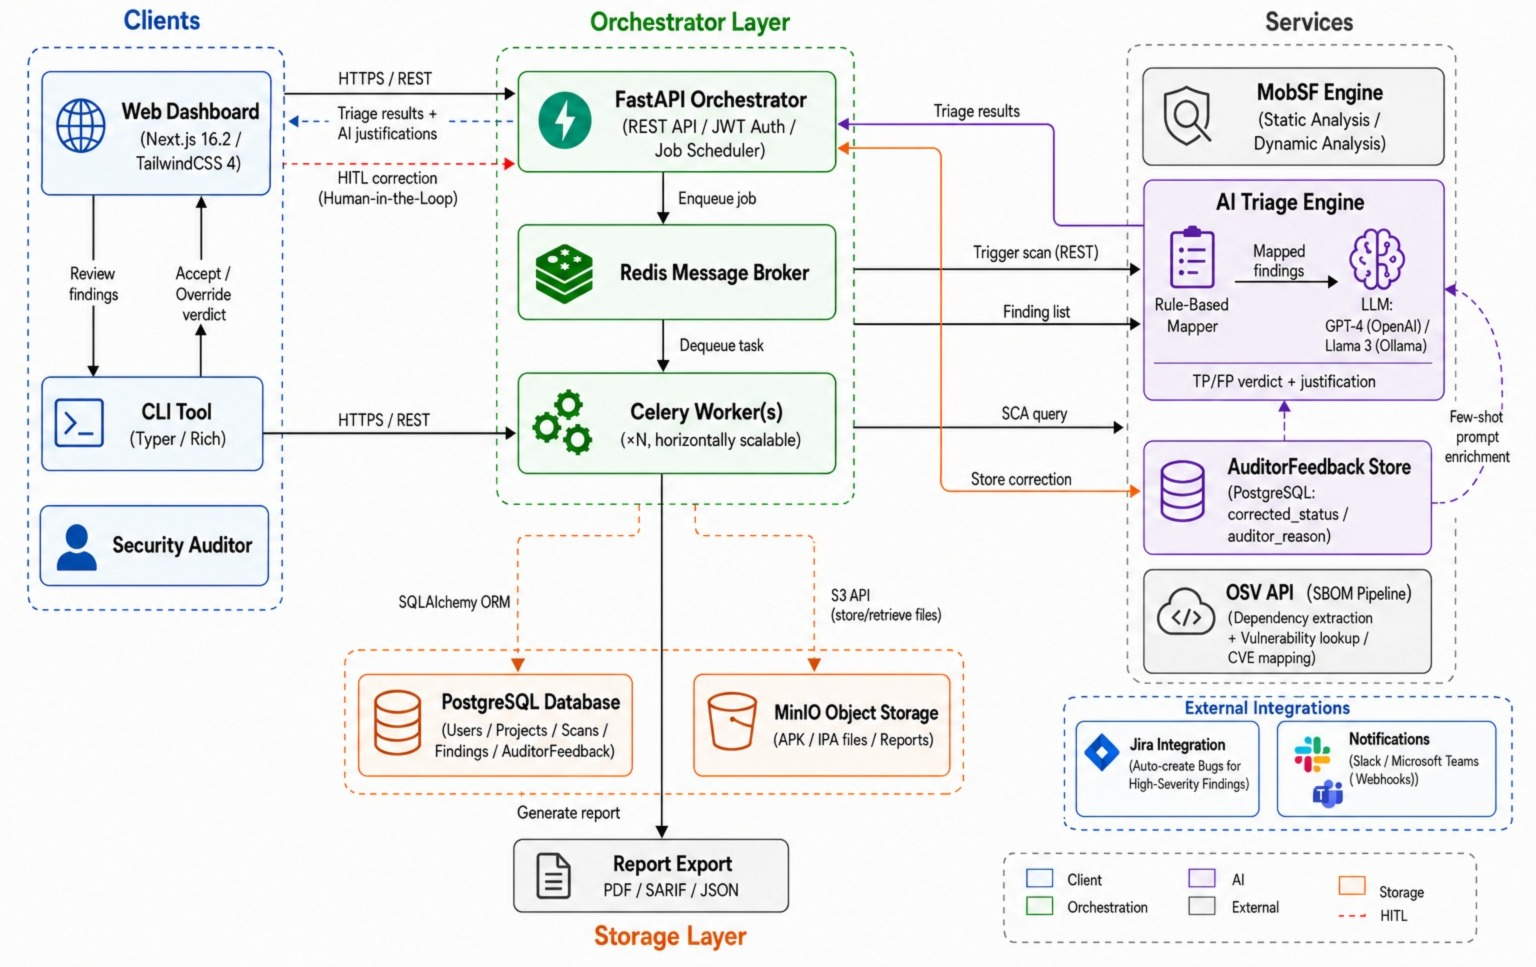
\includegraphics[width=0.95\textwidth]{images/WhatsApp Image 2026-05-09 at 21.09.18 (1).jpeg}
\caption{ThreatLens global software architecture and component interaction. Diagram represents the system architecture at commit \texttt{9c0c173} of the main branch.}
\label{fig:architecture}
\end{figure}

\begin{figure}[!h]
\centering
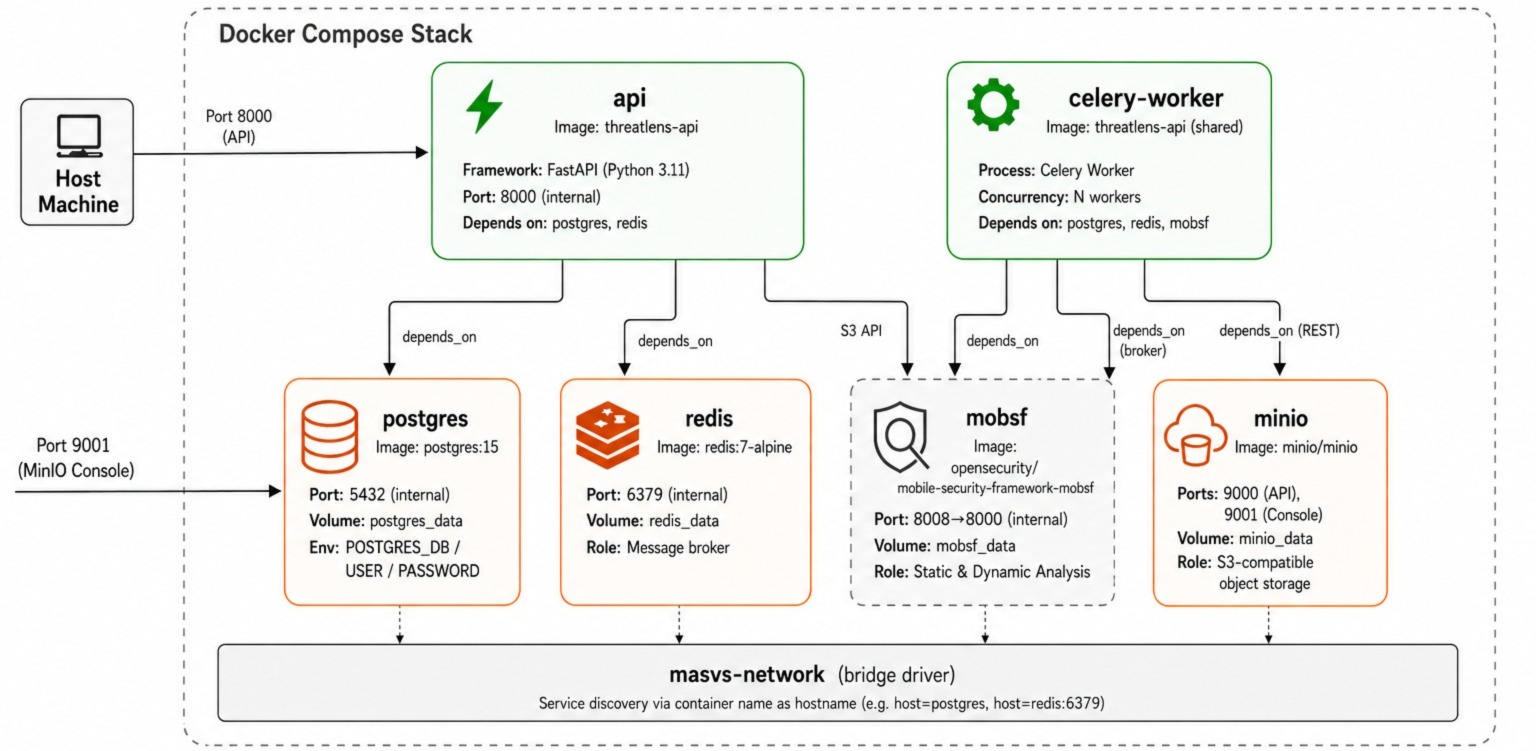
\includegraphics[width=0.95\textwidth]{images/WhatsApp Image 2026-05-09 at 21.09.18.jpeg}
\caption{Docker container orchestration and infrastructure layer (6 services). Diagram reflects the service configuration defined in \texttt{infra/docker-compose.yml} at commit \texttt{9c0c173}, reproducible via \texttt{docker compose up --build -d}.}
\label{fig:docker}
\end{figure}

\subsection{Software functionalities}

ThreatLens exposes the following major functional capabilities.

\begin{enumerate}
  \item \textbf{Automated MASVS v2 mapping.} Each raw finding produced by
    MobSF carries an Androguard tag or a human-readable issue code. The
    mapping engine maintains 61 curated entries associating MobSF issue codes with MASVS v2 controls. Table~\ref{tab:mapping_samples} shows 10 representative entries; the complete mapping dictionary is available in the repository at \texttt{backend/app/mapping/masvs\_mapper.py}. The mapping is fully auditable and can be extended by practitioners to cover organisation-specific rules.

\begin{table}[h]
\caption{Representative entries from the MobSF-to-MASVS v2 mapping table (61 entries total, full table available at \texttt{backend/app/mapping/masvs\_mapper.py})}
\label{tab:mapping_samples}
\begin{tabular}{lll}
\hline
MobSF Issue Code & MASVS v2 Control & Severity \\
\hline
hardcoded\_secret & MASVS-STORAGE-1 & High \\
logging & MASVS-STORAGE-2 & Low \\
weak\_crypto & MASVS-CRYPTO-1 & High \\
clear\_text\_traffic & MASVS-NETWORK-1 & High \\
trust\_all\_certs & MASVS-NETWORK-2 & Critical \\
exported\_component & MASVS-PLATFORM-1 & High \\
webview\_javascript & MASVS-PLATFORM-2 & High \\
sql\_injection & MASVS-CODE-1 & Critical \\
vulnerable\_library & MASVS-CODE-3 & High \\
root\_detection & MASVS-RESILIENCE-2 & Info \\
\hline
\end{tabular}
\end{table}

The correctness of all 61 mapping entries is validated by a dedicated unit test suite located at \texttt{backend/tests/test\_masvs\_mapper.py}, executable via \texttt{pytest backend/tests/ -v}. End-to-end functional validation is performed by the benchmark suite described in Section 3.

  \item \textbf{AI-powered triage.} For each mapped finding, the LLM
    triage engine constructs a structured prompt containing: the MASVS
    control definition, the MobSF finding description, and the relevant
    code snippet (when available). The model returns a TP/FP classification
    with a confidence score and a justification paragraph. The system
    supports both local inference (Ollama / Llama~3, fully air-gapped) and
    cloud inference (OpenAI GPT-4o), selectable per project.

  \item \textbf{Human-in-the-Loop (HITL) feedback.} Auditors can override
    any AI triage decision through the dashboard. Each override is stored in
    the \texttt{AuditorFeedback} table with the original AI classification,
    the corrected status, and the auditor's reasoning. This corpus enables
    few-shot prompt enrichment and, in future releases, fine-tuning of the
    triage model on domain-specific labelled data.

  \item \textbf{CVSS scoring and global compliance grade.} Each confirmed
    finding is assigned a CVSS~v3.1 vector based on the MASVS control
    category and the triage context. The platform aggregates these scores
    into a global security grade (A--F, 0--100 scale), providing
    management-level visibility without requiring technical expertise.

  \item \textbf{Remediation generation.} For every confirmed TP finding,
    the LLM remediation engine generates a language-specific secure code
    fix---Kotlin or Java for Android findings, Swift for iOS findings---
    grounded in the OWASP Mobile Application Security Testing Guide
    (MASTG)~\cite{mastg}. Fixes are displayed inline in the dashboard with
    syntax highlighting.

  \item \textbf{Software Composition Analysis (SCA).} The platform
    extracts third-party library metadata from compiled binaries and queries
    the OSV vulnerability database~\cite{osv_api} to detect known CVEs.
    Results are mapped to \textit{MASVS-CODE-3} and included in the
    compliance report.

  \item \textbf{DevSecOps CLI and CI/CD integration.} The \texttt{threatlens} CLI (built with Typer and Rich) exposes a \texttt{scan run} command that uploads an APK/IPA, polls for results, and exits with a non-zero status code if the security score falls below a configurable threshold. This allows ThreatLens to act as a native security gate in GitHub Actions, GitLab CI, or Jenkins pipelines. Note: While ThreatLens maps findings from MobSF, it does not independently execute Semgrep; coverage of Semgrep findings is provided via MobSF's internal static analysis report integration.

  \item \textbf{Report export.} Completed audits can be exported as
    structured JSON (for downstream tooling), PDF compliance reports (for
    clients and regulators), and SARIF~\cite{sarif} files (for direct
    integration with GitHub Code Scanning).
\end{enumerate}

\begin{figure}[!h]
\centering
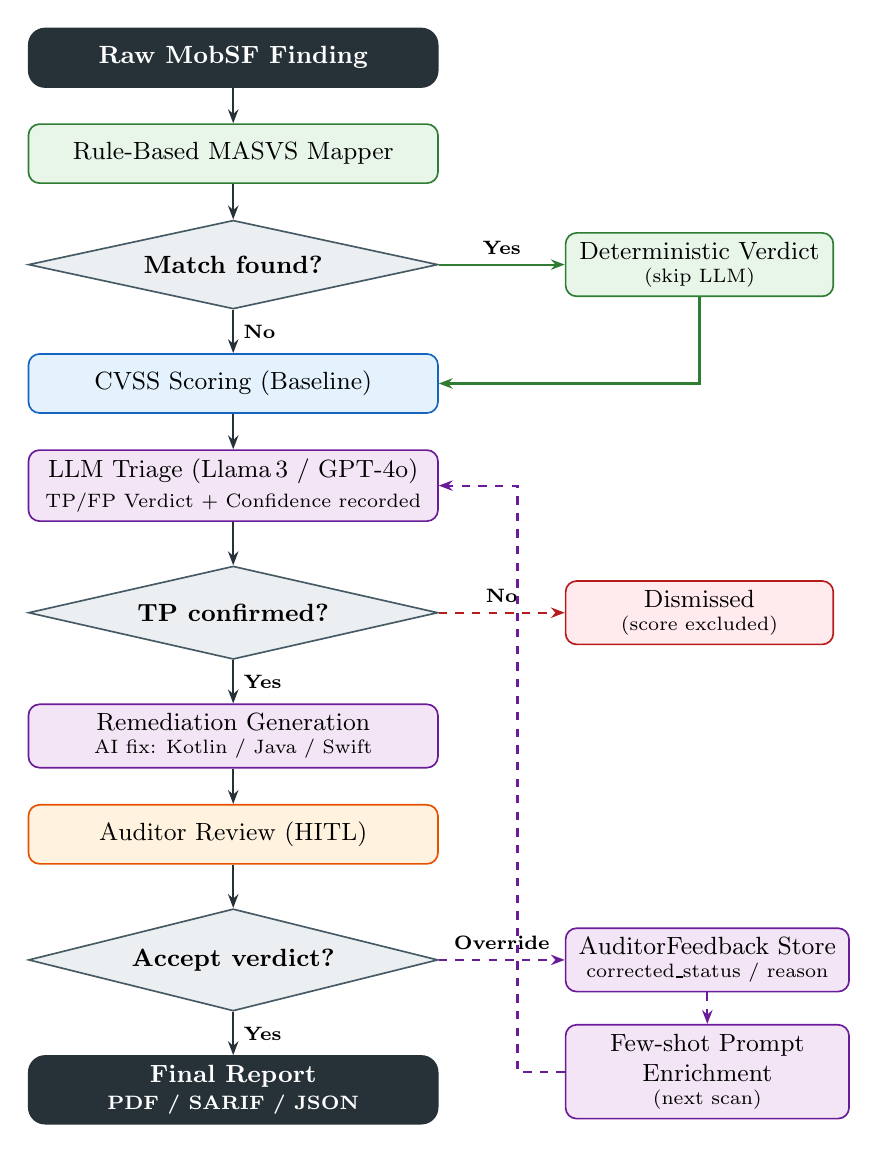
\begin{tikzpicture}[
  %% --- Node styles ---
  startstop/.style={
    rectangle, rounded corners=6pt,
    minimum width=5.2cm, minimum height=0.75cm,
    text centered, font=\small\bfseries,
    fill=tlGrayDark, text=white, draw=tlGrayDark
  },
  process/.style={
    rectangle, rounded corners=4pt,
    minimum width=5.2cm, minimum height=0.75cm,
    text centered, font=\small,
    fill=tlGreenLight, draw=tlGreen, line width=0.6pt
  },
  processAI/.style={
    rectangle, rounded corners=4pt,
    minimum width=5.2cm, minimum height=0.75cm,
    text centered, font=\small,
    fill=tlPurpleLight, draw=tlPurple, line width=0.6pt
  },
  processScore/.style={
    rectangle, rounded corners=4pt,
    minimum width=5.2cm, minimum height=0.75cm,
    text centered, font=\small,
    fill=tlBlueLight, draw=tlBlue, line width=0.6pt
  },
  processHITL/.style={
    rectangle, rounded corners=4pt,
    minimum width=5.2cm, minimum height=0.75cm,
    text centered, font=\small,
    fill=tlOrangeLight, draw=tlOrange, line width=0.6pt
  },
  decision/.style={
    diamond, aspect=2.8,
    minimum width=5.2cm, minimum height=0.9cm,
    text centered, font=\small\bfseries,
    fill=tlGrayLight, draw=tlGray, line width=0.6pt,
    inner sep=1pt
  },
  sidebox/.style={
    rectangle, rounded corners=4pt,
    minimum width=3.4cm, minimum height=0.75cm,
    text centered, font=\small,
    fill=tlRedLight, draw=tlRed, line width=0.6pt
  },
  sideboxGreen/.style={
    rectangle, rounded corners=4pt,
    minimum width=3.4cm, minimum height=0.75cm,
    text centered, font=\small,
    fill=tlGreenLight, draw=tlGreen, line width=0.6pt
  },
  sideboxPurple/.style={
    rectangle, rounded corners=4pt,
    minimum width=3.6cm, minimum height=0.75cm,
    text centered, font=\small,
    fill=tlPurpleLight, draw=tlPurple, line width=0.6pt
  },
  %% --- Arrow style ---
  arrow/.style={-{Stealth[length=5pt]}, line width=0.8pt, draw=tlGrayDark},
  arrowRed/.style={-{Stealth[length=5pt]}, line width=0.8pt, draw=tlRed, dashed},
  arrowPurple/.style={-{Stealth[length=5pt]}, line width=0.8pt, draw=tlPurple, dashed},
  arrowGreen/.style={-{Stealth[length=5pt]}, line width=0.8pt, draw=tlGreen},
  label/.style={font=\scriptsize, midway}
]
 
%% =========================================================
%% NODES — main vertical spine (x=0)
%% =========================================================
\node (start)   [startstop]                          {Raw MobSF Finding};
\node (mapper)  [process,   below=0.45cm of start]   {Rule-Based MASVS Mapper};
\node (dec1)    [decision,  below=0.45cm of mapper]  {Match found?};
\node (cvss)    [processScore, below=0.55cm of dec1] {CVSS Scoring (Baseline)};
\node (llm)     [processAI, below=0.45cm of cvss]
      {\shortstack{LLM Triage (Llama\,3 / GPT-4o)\\{\scriptsize TP/FP Verdict + Confidence recorded}}};
\node (dec2)    [decision,  below=0.55cm of llm]     {TP confirmed?};
\node (remed)   [processAI, below=0.55cm of dec2]
      {\shortstack{Remediation Generation\\{\scriptsize AI fix: Kotlin / Java / Swift}}};
\node (hitl)    [processHITL, below=0.45cm of remed] {Auditor Review (HITL)};
\node (dec3)    [decision,  below=0.55cm of hitl]    {Accept verdict?};
\node (report)  [startstop, below=0.55cm of dec3]
      {\shortstack{Final Report\\{\scriptsize PDF / SARIF / JSON}}};
 
%% =========================================================
%% SIDE NODES — right column
%% =========================================================
\node (detVerdict) [sideboxGreen, right=1.6cm of dec1, yshift=0.0cm]
      {\shortstack{Deterministic Verdict\\{\scriptsize (skip LLM)}}};
 
\node (dismissed)  [sidebox,      right=1.6cm of dec2, yshift=0.0cm]
      {\shortstack{Dismissed\\{\scriptsize (score excluded)}}};
 
\node (feedback)   [sideboxPurple, right=1.6cm of dec3, yshift=0.0cm]
      {\shortstack{AuditorFeedback Store\\{\scriptsize corrected\_status / reason}}};
 
\node (fewshot)    [sideboxPurple, below=0.4cm of feedback]
      {\shortstack{Few-shot Prompt\\Enrichment\\{\scriptsize (next scan)}}};
 
%% =========================================================
%% MAIN SPINE ARROWS
%% =========================================================
\draw[arrow] (start)  -- (mapper);
\draw[arrow] (mapper) -- (dec1);
\draw[arrow] (dec1)   -- node[label, right]{\textbf{No}} (cvss);
\draw[arrow] (cvss)   -- (llm);
\draw[arrow] (llm)    -- (dec2);
\draw[arrow] (dec2)   -- node[label, right]{\textbf{Yes}} (remed);
\draw[arrow] (remed)  -- (hitl);
\draw[arrow] (hitl)   -- (dec3);
\draw[arrow] (dec3)   -- node[label, right]{\textbf{Yes}} (report);
 
%% =========================================================
%% BRANCH ARROWS
%% =========================================================
%% dec1 Yes → Deterministic Verdict (right)
\draw[arrowGreen] (dec1.east)
    -- node[label, above]{\textbf{Yes}} (detVerdict.west);
 
%% Deterministic Verdict feeds into CVSS (skip LLM)
\draw[arrowGreen] (detVerdict.south)
    |- (cvss.east);
 
%% dec2 No → Dismissed (right)
\draw[arrowRed] (dec2.east)
    -- node[label, above]{\textbf{No}} (dismissed.west);
 
%% dec3 No → AuditorFeedback (right)
\draw[arrowPurple] (dec3.east)
    -- node[label, above]{\textbf{Override}} (feedback.west);
 
%% Feedback → Few-shot
\draw[arrowPurple] (feedback) -- (fewshot);
 
%% Few-shot loops back to LLM (curved left side)
\draw[arrowPurple] (fewshot.west)
    -- ++(-0.6,0)
    |- (llm.east);
 
\end{tikzpicture}
\caption{AI triage and remediation workflow (Reproduced from execution at commit 9c0c173). }
\label{fig:ai_workflow}
\end{figure}
\clearpage
\begin{figure}[!h]
\centering
\centering
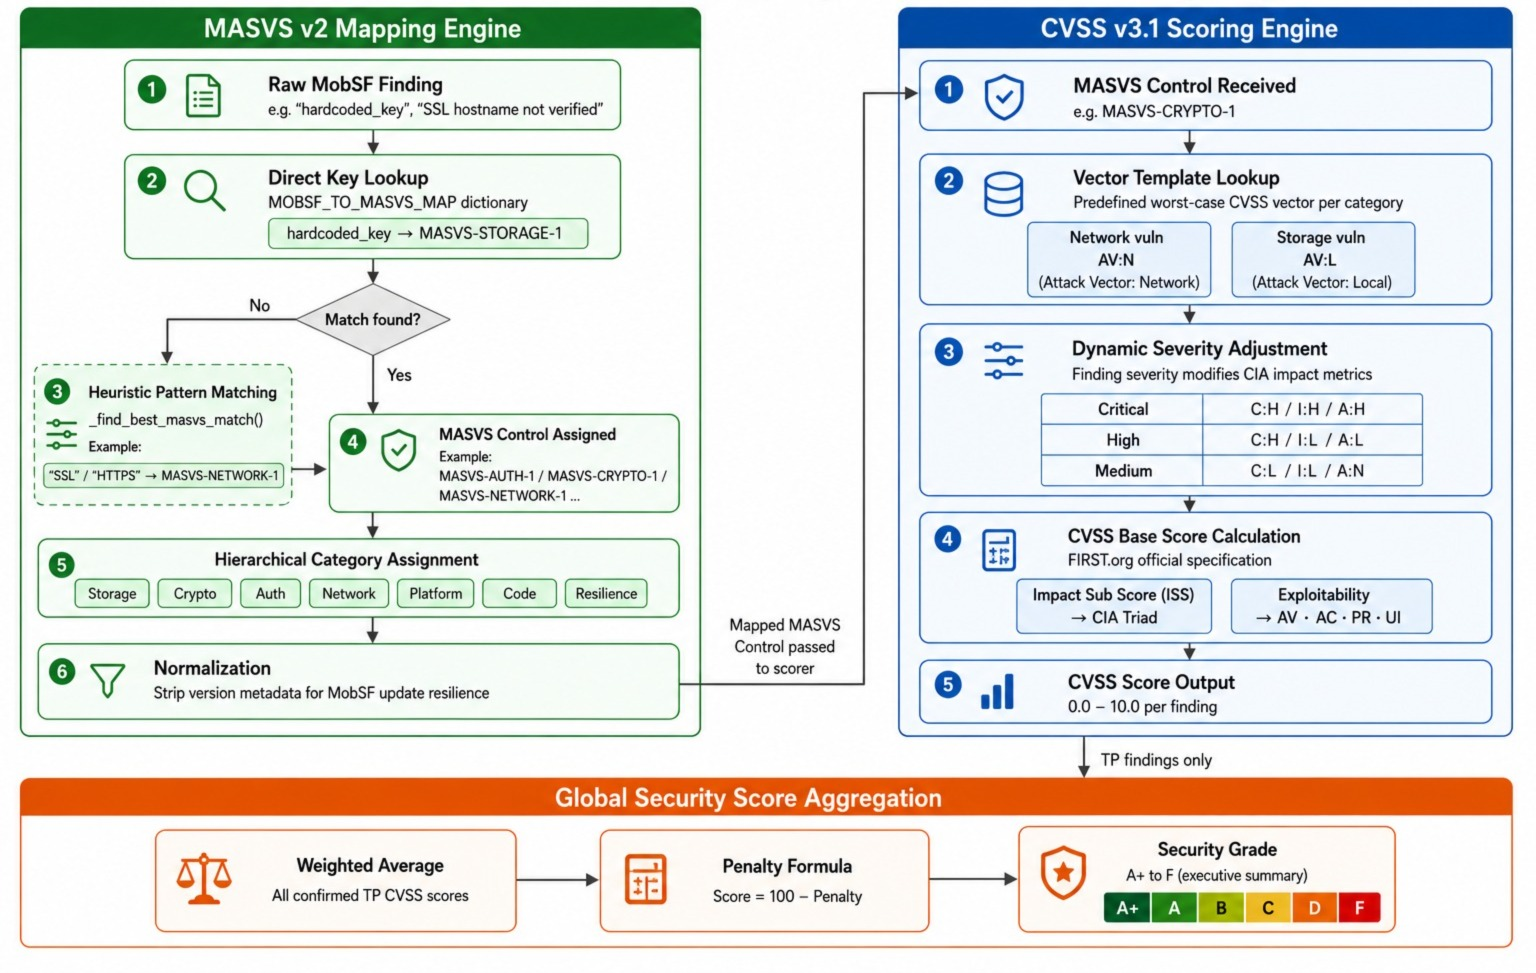
\includegraphics[width=0.95\textwidth]{images/WhatsApp Image 2026-05-09 at 21.07.59.jpeg}
\caption{MASVS v2 compliance mapping and CVSS scoring logic.}
\label{fig:masvs_mapping}
\end{figure}

\subsection{AI triage process}

Algorithm~\ref{alg:triage} summarises the two-pass triage process applied to each
finding $f_i$ in the finding set $F = \{f_1, f_2, \ldots, f_n\}$ returned by MobSF.

\textbf{Pass 1 — Deterministic rule-based mapping.} The system first consults a 
curated mapping table $M$ to assign a MASVS~v2 control identifier $c_i$ and 
an initial technical severity. If a direct match is not found, a heuristic keyword 
matcher performs a second lookup on the finding's title and description. Findings 
that remain unmapped or ambiguous are not discarded but are flagged for 
probabilistic classification in the subsequent pass.

\textbf{Technical Scoring Baseline.} Before AI intervention, each finding is processed 
by the CVSS~v3.1 engine. This ensures that every potential vulnerability has a 
standardized technical score based on its MASVS category and detected severity 
tier $s_i \in \{\text{INFO}, \text{LOW}, \text{MED}, \text{HIGH}, \text{CRITICAL}\}$.

\textbf{Pass 2 — LLM contextual triage.} For findings requiring validation, a 
contextual prompt $p_i$ is constructed:
\[
  p_i = \langle \text{system\_role},\; c_i^{\text{definition}},\; f_i^{\text{description}},\; f_i^{\text{code\_context}} \rangle
\]
and processed by the LLM backend (Ollama/OpenAI). The model returns a structured 
verdict $v_i \in \{\text{TP}, \text{FP}\}$ along with a confidence score 
$\sigma \in [0,1]$ and a natural language justification.
Findings classified as False Positives by the LLM are preserved in the database for audit trail 
integrity but are excluded from the final security score calculation.

\begin{algorithm}
\caption{Two-Pass AI Triage (triage\_findings\_batch)}
\label{alg:triage}
\begin{algorithmic}[1]
\Require $F = \{f_1, \ldots, f_n\}$ (MobSF findings)
\Require $M$ (MASVS mapping table, 61 entries)
\Require $LLM$ (Ollama/Llama 3 or OpenAI/GPT-4o)
\Ensure $R$ (list of TriageDecision objects)

\For{each $f_i \in F$}
    \State $c_i \leftarrow M.\text{lookup}(f_i.\text{code})$
    \If{$c_i = \emptyset$}
        \State flag $f_i$ as \texttt{UNMAPPED}; \textbf{continue}
    \EndIf

    \State \textbf{Pass 1 --- Deterministic}
    \State $v_i \leftarrow \text{rule\_based\_pre\_triage}(f_i,\, \_RULE\_KEYWORDS)$
    \If{$v_i \neq \texttt{AMBIGUOUS}$}
        \State record deterministic verdict; \textbf{continue}
    \EndIf

    \State \textbf{Pass 2 --- LLM Contextual}
    \State $p_i \leftarrow \langle system\_role,\; c_i^{def},\; f_i^{desc},\; f_i^{code}\rangle$
    \State $(v_i, \sigma_i, j_i) \leftarrow LLM.\text{infer}(p_i,\; T=0.1)$
    \If{JSON parse error}
        \State $v_i \leftarrow TP$, $\sigma_i \leftarrow 0.0$
        \State $j_i \leftarrow$ \texttt{"LLM parse error — defaulting to TP"}
    \EndIf

    \If{$v_i = FP$}
        \State persist $f_i$ with \texttt{triage\_result=FALSE\_POSITIVE}
        \State exclude from security score
    \Else
        \State generate\_remediation$(f_i, c_i)$
        \State $R.\text{append}(TriageDecision(v_i, \sigma_i, j_i))$
    \EndIf
\EndFor
\Return $R$
\end{algorithmic}
\end{algorithm}

The triage function accepts as input a list of Finding objects retrieved from the PostgreSQL database after MobSF analysis. Each Finding contains: the raw MobSF issue code, finding title, description, severity tier, and extracted code snippet when available. The function returns a list of \texttt{TriageDecision} objects, each containing four fields: \texttt{is\_true\_positive} (bool), \texttt{confidence} ($\sigma \in [0,1]$), \texttt{justification} (natural language string, max 3 sentences), and \texttt{suggested\_severity} (optional override). False Positive findings are never deleted; they are persisted in the database with \texttt{triage\_result=FALSE\_POSITIVE} to preserve the full audit trail and enable HITL review and reversal.

\textbf{HITL feedback and prompt enrichment.} The final layer consists of the 
Human-in-the-Loop (HITL) interface. Auditors review the $v_i$ verdicts and 
justifications. If an auditor overrides a verdict, the correction is stored in 
the \textit{AuditorFeedback Store}. 

Auditor corrections are stored in the \texttt{AuditorFeedback} table and injected into subsequent triage prompts as few-shot examples. Specifically, the 3 most recent corrections matching the same MASVS control are prepended to the prompt, allowing the LLM to adapt to organisation-specific interpretation of ambiguous findings. This corpus enables continuous improvement of the triage engine without requiring model fine-tuning.

\subsection*{LLM Configuration and Prompt Design}

\textbf{System prompt.} The following role prompt 
is sent to the LLM backend for every triage call:

\begin{quote}
\textit{"You are an expert mobile application 
security auditor specializing in the OWASP MASTG. 
Your task is to analyze security findings from 
automated static analysis and determine if each 
finding is a TRUE POSITIVE (real vulnerability) 
or a FALSE POSITIVE (not exploitable or not 
applicable)."}
\end{quote}

\textbf{Temperature.} A value of $T = 0.1$ is 
used for both the local Ollama/Llama 3 backend 
and the cloud OpenAI/GPT-4o backend. This low 
value minimises output variance and promotes 
deterministic, factual responses suited to 
security auditing.

\textbf{Expected output schema.} The LLM is 
instructed to return exclusively a JSON object 
conforming to the following schema:

\begin{verbatim}
{
  "is_true_positive": boolean,
  "confidence": float (0.0 to 1.0),
  "justification": "string",
  "suggested_severity": "critical|high|medium|
                          low|info|null"
}
\end{verbatim}

\textbf{Hallucination controls.} Output is 
validated via \texttt{json.loads()}. If parsing 
fails, the system retries up to 2 times. After 
3 failed attempts, a conservative fallback 
applies: the finding is marked True Positive 
with $\sigma = 0.0$, forcing mandatory HITL 
review. MASVS control definitions are injected 
verbatim from the mapping table to prevent the 
model from inventing control descriptions.

\textbf{Few-shot prompt enrichment.} Up to 3 
historical auditor corrections are dynamically 
injected into each prompt via 
\texttt{\_historical\_feedback\_text()} in 
\texttt{scan\_tasks.py}. Examples are selected 
as the 3 most recent HITL overrides matching 
the same MASVS control, enabling the model to 
learn from expert decisions on identical 
vulnerability types.

\textbf{Confidence threshold.} No hard 
blocking threshold is currently enforced. 
A confidence of $\sigma = 0.0$ is assigned 
by the system in two cases: (1) LLM parse 
error after retries, and (2) absent code 
snippet context. Both cases serve as a 
visual critical signal in the dashboard 
for mandatory auditor review.

\begin{table}[h]
\caption{LLM triage performance metrics (evaluated on 4-APK corpus, 92 total findings)}
\label{tab:latency}
\begin{tabular}{lll}
\hline
Backend & Mean latency/finding & Total cost \\
\hline
Llama 3 8B (local, Ollama v0.23.2) & 
  13.4 s & \$0.00 \\
GPT-4o (cloud, estimated) & 
  2--4 s & Not tracked \\
\hline
\end{tabular}
\end{table}

\textit{Note: Llama 3 latency derived from 
DivaApplication benchmark (793s / 59 findings). 
GPT-4o latency is an estimate; token costs are 
not systematically logged in the current release. 
Cost tracking is planned for v1.1.}


%%============================================================
\section{Illustrative examples}
%%============================================================

We present two representative usage scenarios to demonstrate ThreatLens in practice.

\subsection{Scenario 1: CI/CD security gate}

A mobile development team integrates ThreatLens into their GitHub Actions pipeline. On every pull request targeting the \texttt{main} branch, the following workflow step is executed on \texttt{UnCrackable-Level1.apk} (OWASP MASTG reference application, SHA-256: \texttt{1da8bf57...dbef96f21}, 0.06 MB), a publicly available intentionally vulnerable Android application maintained by the OWASP Foundation~\cite{owasp_mastg}.

\begin{lstlisting}[language=bash, 
  caption={ThreatLens CLI in a GitHub Actions 
  workflow (UnCrackable-Level1.apk, 
  SHA-256: 1da8bf57d266109f9a07c01bf7111a1975ce01f190b9d914bcd3ae3dbef96f21)},
  label={lst:cli}]
- name: ThreatLens Security Gate
  run: |
    # Verify APK integrity before scan
    echo "1da8bf57d266109f9a07c01bf7111a1975ce01f190b9d914bcd3ae3dbef96f21  UnCrackable-Level1.apk" | sha256sum -c

    threatlens scan run UnCrackable-Level1.apk \
      --project "MSTG-Audit-Evaluation" \
      --fail-on high
\end{lstlisting}

The CLI uploads the APK to the ThreatLens backend, waits for the asynchronous scan
to complete, and prints a Rich-formatted summary to the console. If any findings with 
a severity of \textbf{High} or \textbf{Critical} are detected, the step exits with code~1, 
blocking the pull request merge until the vulnerabilities are resolved or suppressed. 
The SARIF artefact generated by ThreatLens can be automatically downloaded and 
uploaded to GitHub Code Scanning, annotating each vulnerable line of code directly 
in the pull request diff view.

\begin{figure}[!h]
\centering
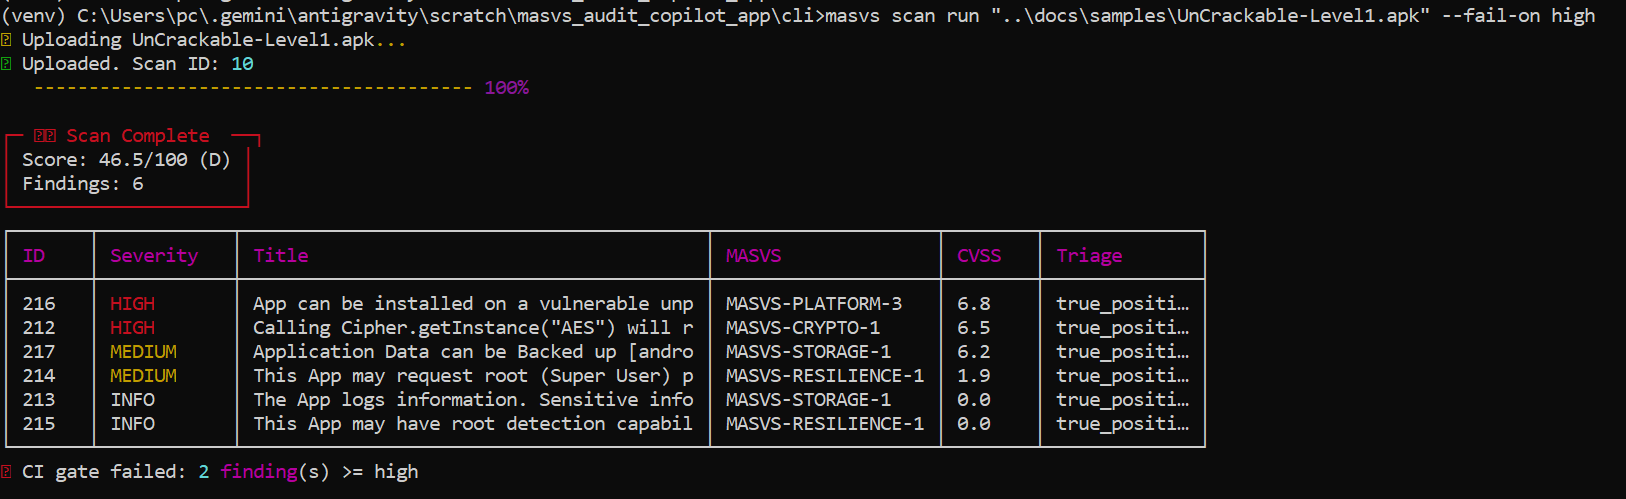
\includegraphics[width=0.95\textwidth]{images/3.png}
\caption{ThreatLens CLI execution and CI/CD security gate output in GitHub Actions (Reproduced from execution at commit 9c0c173). }
\label{fig:cli_cicd}
\end{figure}


\subsection{Scenario 2: Full audit workflow via the web dashboard}

An independent security auditor uploads \texttt{DivaApplication.apk} (Damn Insecure and Vulnerable App v1.0, SHA-256: \texttt{5cefc51f...fab7c5}, 1.43~MB, sourced from~\cite{diva_android}). The scan completes in 793 seconds on a 4-vCPU/16~GB RAM server running Docker 24.0+, producing 59 raw MobSF findings. After LLM triage, 43 are confirmed as True Positives and 16 are classified as False Positives.

The auditor navigates to the \textit{AI Triage} view (Fig.~\ref{fig:dashboard}). Each
finding card displays: the MASVS control it maps to, the AI verdict (TP/FP), the
confidence score, and the LLM-generated justification paragraph. The auditor reviews
a finding flagged as TP under \textit{MASVS-STORAGE-2} (``Sensitive data stored in
cleartext in SharedPreferences''), agrees with the assessment, and clicks
\textit{Accept}. For another finding under \textit{MASVS-NETWORK-1}, the auditor
disagrees with the FP classification---the LLM missed the relevant hostname pinning
bypass---and overrides the verdict to TP, adding a short comment. This correction is
stored in the \texttt{AuditorFeedback} table.

After reviewing all findings, the auditor exports a PDF compliance report and a SARIF
file, which are delivered to the development team.

\begin{figure}[!h]
\centering
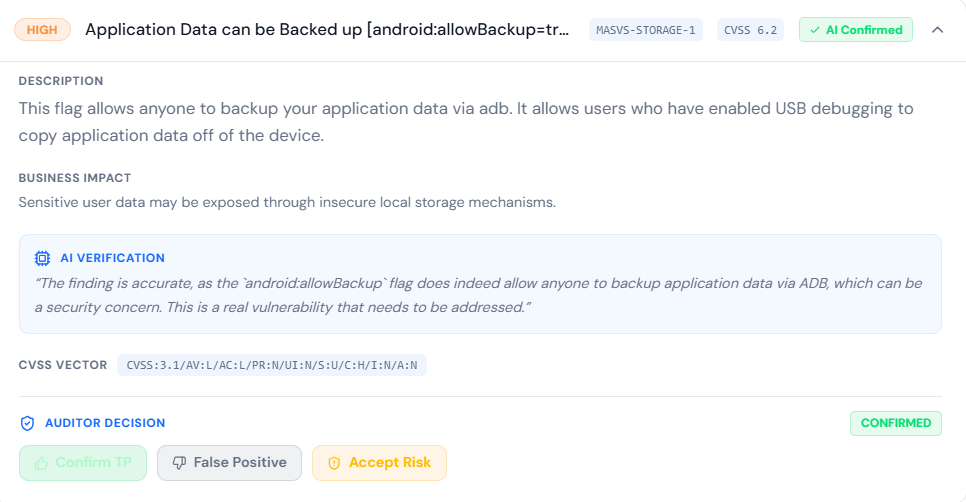
\includegraphics[width=0.95\textwidth]{images/8.png}
\caption{ThreatLens compliance dashboard showing MASVS category coverage and AI-triaged finding list (Reproduced from execution at commit 9c0c173). }
\label{fig:dashboard}
\end{figure}

%%============================================================
\section{Experimental Evaluation}
%%============================================================

To evaluate the performance and reliability of ThreatLens, we conducted an experimental
assessment using a reproducible corpus of public Android applications. The evaluation
answers three questions: whether AI triage preserves vulnerability signal after raw MobSF
analysis, how much manual audit effort is reduced, and which MASVS v2 areas are covered
by the benchmark corpus.

\subsection{Evaluation Protocol}

All scans were executed on a standardized Ubuntu 22.04 environment with 4 vCPUs,
16~GB RAM, Docker 24.0+, Docker Compose v2.24+, MobSF v3.9.7, and Llama~3 8B
Instruct served through local Ollama. ThreatLens was executed at commit
\texttt{9c0c173}; scan durations were measured from the \texttt{started\_at} and
\texttt{completed\_at} timestamps persisted by the \texttt{Scan} model.

The APK corpus contains four intentionally vulnerable public Android applications:
DIVA, InsecureBankv2, and two OWASP MASTG UnCrackable crackmes. Table~\ref{tab:dataset}
lists the exact dataset metadata used for reproduction, including APK size and SHA-256
hashes from \texttt{benchmark/data.csv}.

Ground-truth labels were established by comparing raw AI verdicts from
\texttt{benchmark/results/summary.csv} with the labelled benchmark file
\texttt{benchmark/ground\_truth.json}. Manual baseline times were recorded in
\texttt{benchmark/audit\_logs.csv} by a Senior Security Engineer performing full MASVS
v2 finding review, control mapping, severity assessment, and report note drafting.
As discussed in the limitations, the manual baseline uses a single auditor and should be
interpreted as indicative rather than statistically generalizable.

\subsection{Dataset Characteristics}

\begin{table}[!h]
\caption{Evaluation APK corpus from \texttt{benchmark/data.csv}}
\label{tab:dataset}
\centering
\scriptsize
\resizebox{\textwidth}{!}{%
\begin{tabular}{lllll}
\hline
APK & Version & Type & Size (MB) & SHA-256 \\
\hline
DivaApplication & 1.0 & Vulnerable & 1.43 & \texttt{5CEFC51FCE9BD760B92AB2340477F4DDA84B4AE0C5D04A8C9493E4FE34FAB7C5} \\
InsecureBankv2 & 1.0 & Vulnerable & 3.30 & \texttt{B18AF2A0E44D7634BBCDF93664D9C78A2695E050393FCFBB5E8B91F902D194A4} \\
UnCrackable-Level1 & 1.0 & CTF & 0.06 & \texttt{1DA8BF57D266109F9A07C01BF7111A1975CE01F190B9D914BCD3AE3DBEF96F21} \\
UnCrackable-Level3 & 1.0 & CTF & 1.39 & \texttt{6827F776B7D2844342711BE6F13695AE8D1A5F209FC0072DBAF8B85E2FCFF4B7} \\
\hline
\end{tabular}
}
\end{table}

The corpus produced 92 raw findings across the four APKs. These findings covered
9 unique MASVS v2 controls out of 41 total controls in MASVS v2; the current mapping
engine supports 17 unique controls. Table~\ref{tab:masvs_coverage} summarizes the
available per-category coverage. A finding-level per-MASVS TP/FP confusion matrix was
not available in the benchmark artifacts, so category results are reported as coverage
rather than accuracy.

\begin{table}[!h]
\caption{MASVS v2 category coverage observed in the 4-APK corpus}
\label{tab:masvs_coverage}
\centering
\begin{tabular}{lll}
\hline
MASVS Category & Controls observed & APKs covered \\
\hline
AUTH & MASVS-AUTH-1 & 1/4 \\
CODE & MASVS-CODE-1, MASVS-CODE-2 & 2/4 \\
CRYPTO & MASVS-CRYPTO-1 & 1/4 \\
PLATFORM & MASVS-PLATFORM-1, MASVS-PLATFORM-3 & 4/4 \\
RESILIENCE & MASVS-RESILIENCE-1, MASVS-RESILIENCE-3 & 3/4 \\
STORAGE & MASVS-STORAGE-1 & 4/4 \\
\hline
\end{tabular}
\end{table}

\subsection{Triage Performance}

The benchmark distinguishes raw AI triage verdicts from post-validation evaluation labels. Raw verdict totals are taken from \texttt{benchmark/results/summary.csv}: 75 findings were classified by the AI as True Positive and 17 as False Positive. The confusion matrix below is computed by comparing those raw verdicts against the labelled benchmark file \texttt{benchmark/ground\_truth.json}: 67 of the 75 AI-positive verdicts remained True Positives, while 8 were counted as False Positives; among the 17 AI-negative verdicts, 14 were confirmed as True Negatives and 3 were counted as False Negatives. As noted in the limitations, no fabricated comparison data against standalone MobSF or Semgrep was used for this benchmark.

\begin{table}[!h]
\centering
\begin{tabular}{lr}
\toprule
\textbf{Metric} & \textbf{ThreatLens} \\
\midrule
Total Findings Analyzed  & 92 \\
AI Positive Verdicts (raw AI TP) & 75 \\
AI Negative Verdicts (raw AI FP) & 17 \\
True Positives (AI TP / labelled TP) & 67 \\
False Positives (AI TP / labelled FP) & 8 \\
False Negatives (AI FP / labelled TP) & 3 \\
True Negatives (AI FP / labelled FP) & 14 \\
\textbf{Precision}       & \textbf{89.33\%}* \\
\textbf{Recall}          & \textbf{95.71\%} \\
\textbf{F1-Score}        & \textbf{92.41\%} \\
Mean Scan Time (sec)     & 308.75 \\
Mean Speedup vs Manual   & \textbf{9.2x} \\
\bottomrule
\end{tabular}
\caption{Performance on a corpus of 4 public APKs. (*) Precision, recall, and F1 are computed from the benchmark confusion matrix in \texttt{ground\_truth.json}; raw AI verdict totals come from \texttt{summary.csv}.}
\label{tab:evaluation}
\end{table}

\subsection{Time Efficiency}

ThreatLens reduced mean MASVS compliance report generation time from 47.5 minutes
for the manual baseline to 5.1 minutes for the automated pipeline. Across the 4-APK
corpus, total effort decreased from 190 minutes to 20.6 minutes, corresponding to a
mean speedup of $9.2\times$. Table~\ref{tab:time_comparison} presents the per-APK
breakdown.

\begin{table}[!h]
\caption{Audit time comparison: manual baseline vs. ThreatLens automated pipeline (4-APK corpus)}
\label{tab:time_comparison}
\centering
\begin{tabular}{lllll}
\hline
APK & Manual (min) & ThreatLens (sec) & ThreatLens (min) & Speedup \\
\hline
DivaApplication & 126.0 & 793 & 13.2 & 9.5$\times$ \\
InsecureBankv2 & 24.0 & 188 & 3.1 & 7.7$\times$ \\
UnCrackable-L1 & 11.0 & 75 & 1.2 & 8.8$\times$ \\
UnCrackable-L3 & 29.0 & 179 & 3.0 & 9.7$\times$ \\
\hline
\textbf{Total} & \textbf{190.0} & \textbf{1,235} & \textbf{20.6} & \textbf{9.2$\times$} \\
\hline
\end{tabular}
\end{table}

\textit{ThreatLens times exclude HITL review. Auditor validation of AI-triaged findings
requires an estimated 15--45 seconds per finding, compared with several minutes per
finding during fully manual classification from zero.}

%%============================================================
\section{Impact}
%%============================================================

\subsection{Scientific and research impact}

ThreatLens enables new research questions that were previously difficult to study at scale.
By providing a platform that collects structured, labelled triage data (AI verdict +
human correction), it enables empirical benchmarking of different LLM backends on the
specialised task of mobile vulnerability classification. This addresses an open gap in the
literature: while studies such as~\cite{llm_vuln} demonstrate LLM capability in general
code review, performance on narrow compliance domains (MASVS, PCI-DSS, GDPR) is
understudied. The \texttt{AuditorFeedback} corpus generated by ThreatLens deployments
is a novel labelled dataset that researchers can use for fine-tuning, few-shot learning,
or evaluation of future security-focused language models.

The platform also provides a reproducible, version-controlled environment for mobile
security research. Researchers can pin a specific combination of MobSF version, LLM
backend, and MASVS mapping ruleset, then run identical scans on a benchmark APK
corpus to obtain comparable results across studies.

\subsection{Practical and industrial impact}

For security practitioners, ThreatLens changes the daily audit workflow in three
concrete ways. First, as shown in Table~\ref{tab:time_comparison}, ThreatLens reduces
mean MASVS compliance report generation time from 47.5 minutes (manual baseline,
Senior Security Engineer) to 5.1 minutes (automated pipeline), a mean speedup of
$9.2\times$ across the 4-APK evaluation corpus.

Beyond automated processing time, HITL auditor review of AI-triaged findings requires an estimated 15--45 seconds per finding (reading the LLM justification and validating the code context), compared to several minutes per finding during fully manual classification from zero. For the DivaApplication corpus (43 confirmed TPs), this represents an estimated additional 11--32 minutes of expert review time, bringing the total ThreatLens workflow (automated + HITL) to approximately 24--46 minutes versus 126 minutes manual, a conservative $2.7$--$5.3\times$ speedup even accounting for human oversight.

\textbf{Measurement methodology.} Manual audit times were recorded by a single Senior Security Engineer using task-timing software. Times include: finding review, MASVS v2 control mapping, severity assessment, and report note drafting. They exclude initial APK download and environment setup. As measurements were conducted by a single auditor without a control group, inter-auditor variability is not captured; results should be interpreted as indicative rather than statistically generalizable.

For organisations, ThreatLens offers an open-source, self-hostable alternative to
expensive commercial platforms. Sensitive APKs never leave the organisation's
infrastructure when using the local Ollama/Llama~3 backend, which is critical for
enterprises subject to data residency regulations. The modular architecture also
allows integration with existing SIEM and ticketing systems (e.g.\ Jira, Splunk)
through the JSON export API.

\subsection{Comparison with existing tools}

Table~\ref{tab:comparison} positions ThreatLens against primary alternatives, incorporating both architectural capabilities and empirical finding reduction observed during the 4-APK benchmark.

\begin{table}[h]
\caption{Comparison of ThreatLens with existing mobile security tools. Quantitative metrics are derived from execution on the 4-APK public evaluation corpus (DivaApplication, InsecureBankv2, UnCrackable L1, and UnCrackable L3). Architectural capabilities are based on official documentation.}
\label{tab:comparison}
\centering
\begin{tabular}{lcccc}
\hline
Feature / Metric & MobSF & Semgrep & NowSecure & ThreatLens \\
\hline
\multicolumn{5}{l}{\textit{Architectural capabilities}} \\
Static analysis & \checkmark & \checkmark & \checkmark & \checkmark \\
Dynamic analysis & \checkmark & $\times$ & \checkmark & \checkmark \\
MASVS v2 auto-mapping & $\times$ & $\times$ & Partial & \checkmark \\
LLM-assisted triage & $\times$ & $\times$ & Partial & \checkmark \\
HITL feedback loop & $\times$ & $\times$ & \checkmark & \checkmark \\
CVSS v3.1 auto-scoring & $\times$ & $\times$ & Partial & \checkmark \\
AI remediation generation & $\times$ & $\times$ & \checkmark & \checkmark \\
CI/CD native integration & Partial & \checkmark & \checkmark & \checkmark \\
SARIF export & $\times$ & \checkmark & Partial & \checkmark \\
Open-source & \checkmark & \checkmark & Partial & \checkmark \\
\hline
\multicolumn{5}{l}{\textit{Empirical benchmark results (4-APK corpus)}} \\
Raw findings analyzed & 92 & N/A & N/A & 92 \\
AI positive verdicts & --- & N/A & N/A & 75 \\
AI negative classifications & --- & N/A & N/A & 17 (18.5\%) \\
Precision & --- & N/A & N/A & 89.33\% \\
Recall & --- & N/A & N/A & 95.71\% \\
F1-score & --- & N/A & N/A & 92.41\% \\
Mean processing time & $\sim$4 min & N/A & N/A & 5.1 min \\
MASVS controls identified & N/A & N/A & N/A & 9/41 \\
\hline
\end{tabular}

\vspace{0.3em}

\footnotesize{
ThreatLens uses MobSF as its underlying static and dynamic analysis engine; therefore, raw finding counts are identical before AI-assisted triage. Semgrep was not independently benchmarked because it operates primarily on source code rather than compiled APK binaries, making direct APK-level comparison methodologically incompatible in this study.
NowSecure features are based on official documentation. No empirical comparison was performed as NowSecure requires a commercial license.
}
\end{table}



\section{Limitations and Future Work}

\subsection{Limitations}

The following limitations should be considered when interpreting the results of this study:

\begin{enumerate}
\item Corpus size: The evaluation corpus comprises 4 intentionally vulnerable APKs. Results may not generalize to production applications with different code patterns.
\item Manual audit baseline: Manual audit times were recorded by a Senior Security Engineer during a single-auditor benchmark run. While this provides a real-world baseline, it does not capture inter-auditor variability or cognitive load, which would require a larger-scale user study.
\item Cross-tool comparison: Comparison against MobSF is based on raw vs. triaged finding counts on identical APKs. Comparison against Semgrep and NowSecure remains architectural, as these tools require different input formats or commercial licenses incompatible with direct APK-level benchmarking in this study.
\item Sequential triage bottleneck: Findings are processed one by one through the LLM. For APKs with many findings (e.g., DivaApplication: 59 findings, 793 seconds), this creates a significant latency. Parallel batch inference is planned for v1.1.
\item \textbf{Error handling conservatism}: When the LLM returns malformed JSON after 2 retries, the system defaults to True Positive with $\sigma = 0.0$. This conservative fallback minimises missed vulnerabilities but may inflate the False Positive rate in edge cases. All such fallback decisions are flagged for mandatory HITL review.
\item \textbf{LLM confidence scores} are not calibrated probabilities and should not be interpreted as statistical confidence intervals.
\item MobSF dependency: ThreatLens inherits all limitations of MobSF's static analysis engine, including limited obfuscation handling.
\end{enumerate}

\subsection{Future Work}

Future work will focus on: (1) expanding dynamic instrumentation capabilities to cover
MASVS runtime controls currently assessed only through static proxies; (2) integrating
a decentralised audit log on an L2 blockchain for non-repudiable compliance evidence;
(3) implementing automated few-shot prompt optimization; and (4) extending SCA coverage to detect supply chain attacks; and (5) implementing per-scan token cost tracking for cloud LLM backends (GPT-4o), with a cost estimate displayed in the dashboard before scan execution to help practitioners choose between local and cloud inference.


%%============================================================
\section{Conclusions}
%%============================================================

ThreatLens represents a significant step toward fully automated, standards-compliant
mobile security auditing. By combining MobSF-based static and dynamic analysis with
a hybrid LLM triage engine, automated MASVS v2 mapping, CVSS scoring, and
AI-generated remediation, the platform addresses the two primary bottlenecks in modern
mobile security audits: alert fatigue and compliance mapping overhead. The Human-in-the-Loop
feedback mechanism ensures expert oversight and legal defensibility, while simultaneously
building a labelled dataset that enables continuous improvement of the AI triage engine.

The open-source, self-hostable architecture makes ThreatLens accessible to small security
teams and independent researchers who cannot afford commercial managed platforms. Its
native CI/CD integration shifts security left, embedding compliance verification into the
development workflow rather than treating it as a release-time activity.

\section*{Acknowledgements}

The authors thank the open-source communities behind OWASP, MobSF, Ollama, and the
OSV project for providing the standards, tools, and data that underpin ThreatLens.

%%============================================================
\begin{thebibliography}{00}

\bibitem{owasp_masvs}
OWASP Foundation, ``Mobile Application Security Verification Standard (MASVS) v2.0,''
2023. [Online]. Available: \url{https://mas.owasp.org/MASVS/}

\bibitem{mastg}
OWASP Foundation, ``Mobile Application Security Testing Guide (MASTG),''
2024. [Online]. Available: \url{https://mas.owasp.org/MASTG/}

\bibitem{mobsf}
A. Abraham,
``MobSF: Mobile Security Framework,''
GitHub Repository, 2024.
[Online]. Available:
\url{https://github.com/MobSF/Mobile-Security-Framework-MobSF}

\bibitem{osv_api}
Google Open Source Security Team,
``OSV.dev: Open Source Vulnerabilities Database,''
2024. [Online]. Available: \url{https://osv.dev/}

\bibitem{alert_fatigue}
R. Vaarandi and M. Pihelgas, ``Using Security Logs for Collecting and Reporting
Technical Security Metrics,'' in \textit{Proc. IEEE Military Communications Conference
(MILCOM)}, pp. 294--299, 2014.

\bibitem{llm_vuln}
H. Pearce, B. Ahmad, B. Tan, B. Dolan-Gavitt, and R. Karri,
``Asleep at the Keyboard? Assessing the Security of GitHub Copilot's Code Contributions,''
in \textit{Proc. IEEE Symposium on Security and Privacy (S\&P)}, 2022,
pp. 754--768, doi:10.1109/SP46214.2022.9833571.

\bibitem{sarif}
Microsoft, ``Static Analysis Results Interchange Format (SARIF) v2.1.0,''
OASIS Standard, 2022. [Online]. Available: \url{https://docs.oasis-open.org/sarif/sarif/v2.1.0/}

\bibitem{sonarqube}
SonarSource, ``SonarQube Documentation,'' 2024.
[Online]. Available: \url{https://docs.sonarsource.com/sonarqube/}

\bibitem{fastapi}
S. Ram\'irez, ``FastAPI,'' 2024.
[Online]. Available: \url{https://fastapi.tiangolo.com/}

\bibitem{celery}
Celery Project, ``Celery: Distributed Task Queue,'' 2024.
[Online]. Available: \url{https://docs.celeryq.dev/}

\bibitem{diva_android}
Payatu Technologies, ``DIVA Android: Damn Insecure and Vulnerable App for Android,'' 2016. [Online]. Available: \url{https://github.com/payatu/diva-android}

\bibitem{owasp_mastg}
OWASP Foundation, ``OWASP Mobile Application Security Testing Guide (MASTG),'' 2024. [Online]. Available: \url{https://mas.owasp.org/MASTG/}

\bibitem{owasp_llm}
OWASP Foundation,
``OWASP Top 10 for Large Language Model Applications,''
2025.
[Online]. Available:
\url{https://owasp.org/www-project-top-10-for-large-language-model-applications/}
\end{thebibliography}

%%============================================================
\section*{Current executable software version}
%%============================================================

\begin{table}[!h]
\centering
\begin{tabular}{|l|p{5.5cm}|p{6.5cm}|}
\hline
\textbf{Nr.} & \textbf{Code metadata description} & \textbf{Information} \\
\hline
S1 & Current software version & v1.0.0 \\
\hline
S2 & Hardware requirements &
4 vCPUs, 8\,GB RAM minimum (16\,GB recommended for MobSF dynamic analysis);
20\,GB free disk space \\
\hline
S3 & Software requirements &
Docker 24+, Docker Compose v2 (all other dependencies are containerised) \\
\hline
S4 & Installation command &
\texttt{git clone https://github.com/hibalahrouf
/ThreatLense.git \&\& docker compose up -{}-build -d} \\
\hline
S5 & Benchmark reproduction command &
\texttt{python benchmark/run\_benchmark.py} \\
\hline
S6 & Public evaluation dataset &
\texttt{docs/samples/*.apk} (4 public APKs with verified SHA-256 hashes) \\
\hline
S7 & Environment configuration &
\texttt{.env.example} provided in repository root \\
\hline
S8 & Reproducible deployment command &
\texttt{docker compose up --build -d} \\
\hline
S9 & Support email for questions & hibalahrouf@gmail.com \\
\hline
\end{tabular}
\caption{Software metadata (mandatory)}
\label{tab:software_metadata}
\end{table}

\end{document}
\endinput
